\chapter{Drone Simulator}
\lhead{\thechapter \space Drone Simulator}
\label{ch:simulator}

%Header
This chapter describes the current state of the simulation, the preliminary research done, and the planning regarding further improvements.

\section{Preliminary Research}
\label{sec:sim_research}
As testing on live drones is generally not desired due to potential damaging costs and limited battery life, there was opted for a simulation.\hfil
\\\\
When it comes to simulations, drones are commonly-used objects. With this in mind, the initial plan was to reuse an existing project. Since the collision avoidance algorithm will most likely to be developed using Python, it would be ideal to make use of a Python-native simulation. Ultimately, this led to project PyQuadSim by Github user "simondlevy". \cite{simon_github} \hfil
\begin{figure}[h]
	\centering
	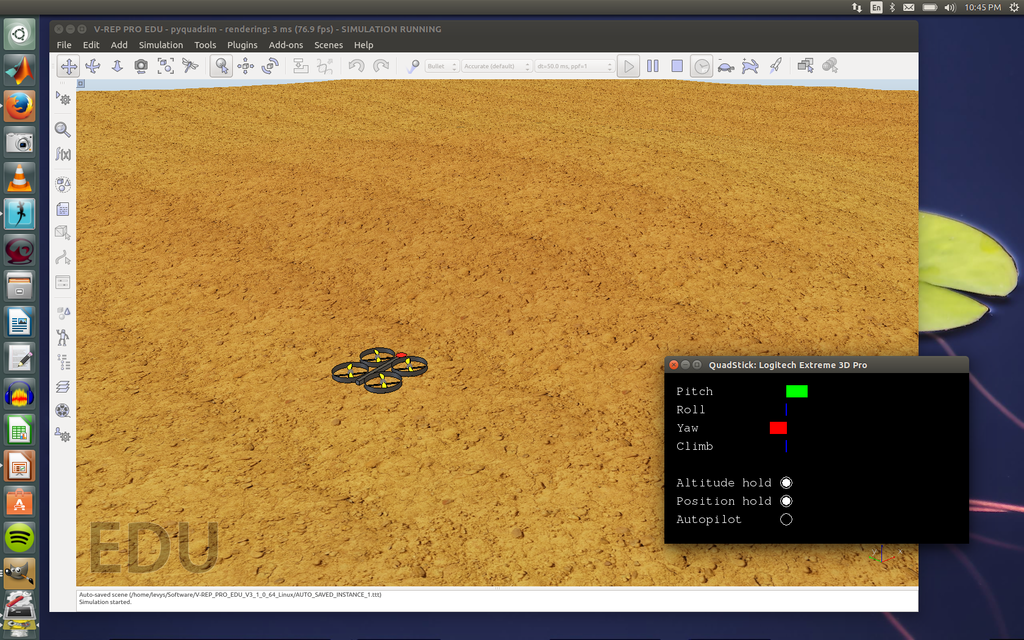
\includegraphics[width=\linewidth]{img/pyquadsim.png}
	\caption{The PyQuadSim project running. \cite{pyquadsim}}
	\label{fig:pyquadsim}
\end{figure}

\noindent
One of the biggest problems of using most \gls{AI} algorithms, is transferring its knowledge to the real application. In the case of for example reinforcement learning, there are generally 2 approaches possible when it comes to real life applications: Train it in the real life environment, or use a simulation with transfer learning. Same as with this project, the former is often too expensive and come with too many risks. However, while simulations are the safer option, they come with the risk of not providing an identical environment. As it is difficult to determine or guide the algorithm on what states which actions should be taken, chances are that the algorithm will react improperly in the real environment if the simulation was not realistic enough. With this in mind, it was decided to look elsewhere for a solution that could provide a simulation more tailored to this case.
\\\\
Based on the arguments above and on the advice from the company supervisor it was decided to develop a new simulation. The Unity game engine was chosen since it is easy to pick up, and 3D models for both the drone and the warehouse were available.

\section{Current State}
\label{sec:sim_status}
As of writing this document, a simulation has been made using Unity. It is capable of generating a variably-sized warehouse with interior and targets. It is designed to be controlled from the first person perspective of the drone, with as goal to collect the targets in the warehouse before the timer runs out.
\begin{figure}[h]
	\centering
	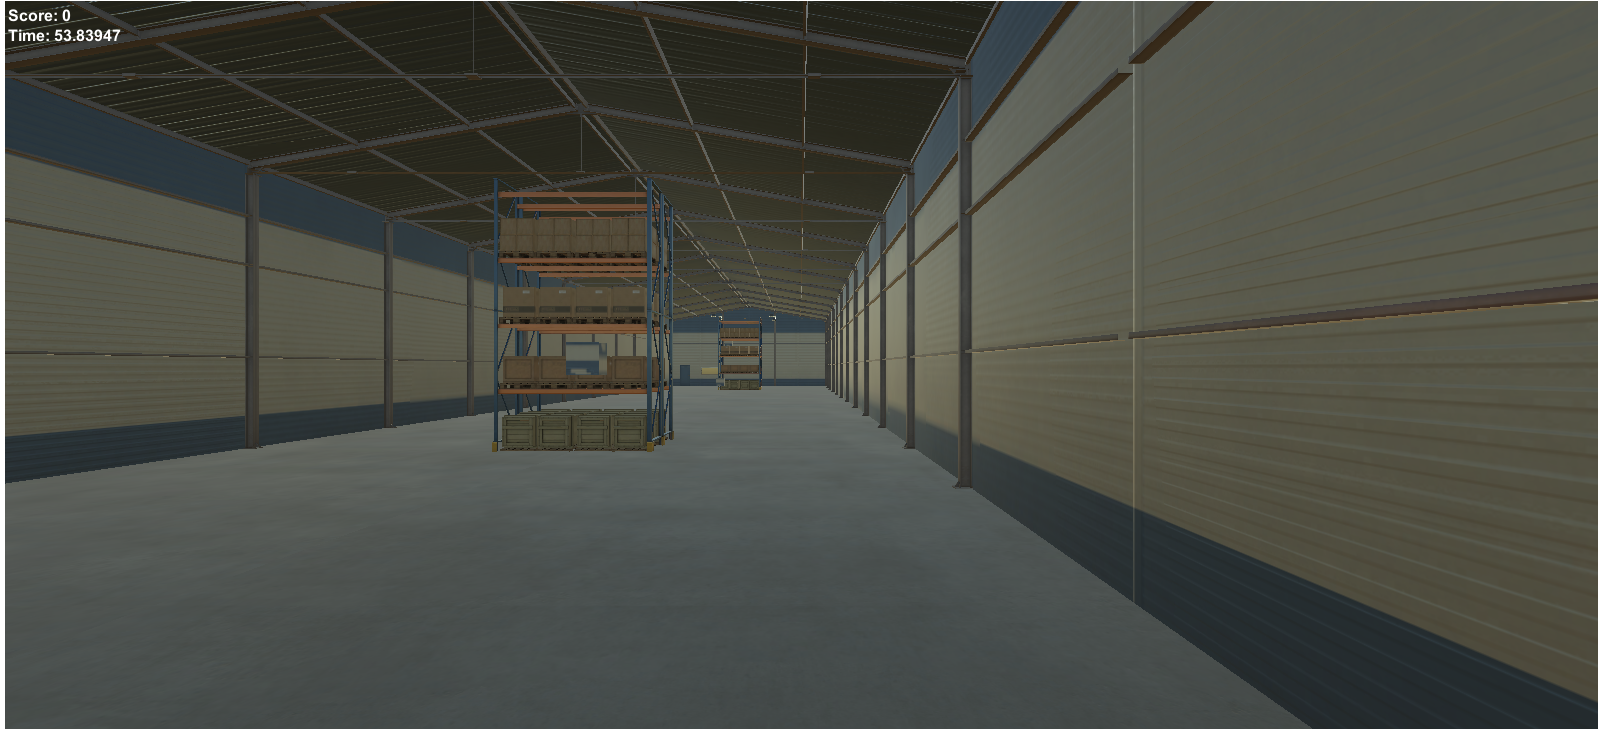
\includegraphics[width=\linewidth]{img/unity_drone.png}
	\caption{Screenshot of the Unity simulator gameplay.}
	\label{fig:unity_drone}
\end{figure}
\pagebreak
\noindent
When training an algorithm the simulation should run at an increased speed. To facilitate this, a training mode has also been added to the simulation. This mode cuts out most of the aesthetics in order to decrease processing overhead. Using this in combination with running the game in a small resolution window should allow for faster game speeds.

\begin{figure}[h]
	\centering
	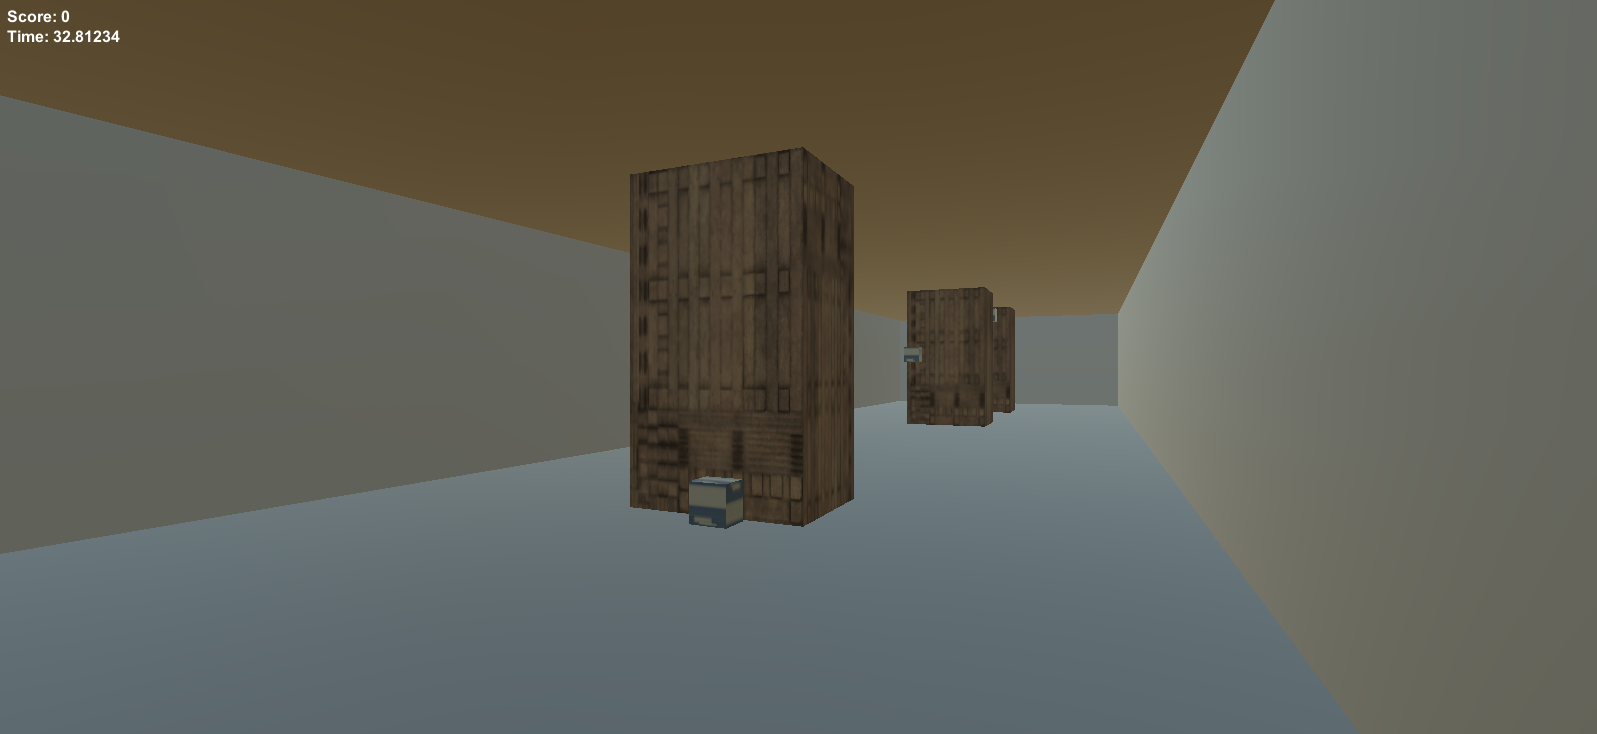
\includegraphics[width=\linewidth]{img/unity_drone_training.png}
	\caption{The Unity simulator in training mode.}
	\label{fig:unity_training}
\end{figure}

\noindent
The implementation of the simulation contains 4 major parts: generator classes, the Unity package, the ML-Agents package and its inheriting classes, and the class for reading a configuration file. Since the Unity package is the default package that all c\# Unity projects use, it will not be discussed here. A class diagram can be found in appendix \ref{app:sim_class_diagram};

\paragraph{Generator} Generator is an abstract class that has concrete implementations for spawning the drone, warehouse, and the targets. Using the strategy design pattern, all the generators are registered and invoked by the DroneAcademy class.

\paragraph{DroneAcademy} DroneAcademy inherits from the Academy class within the ML-Agents package. It is responsible for all operations around the environment during training, for example destroying or adding new objects to the scene. \cite{mlagents_github}

\paragraph{DroneAgent} DroneAgent inherits from the Agent class within the ML-Agents package. The object containing an implementation of the Agent class is meant to be controlled by a neural network (or "brain" in the context of Unity) during training. \cite{mlagents_github}

\paragraph{ConfigHandler} ConfigHandler reads an external configuration file that contains information about how to generate the scene. Examples include the size of the warehouse and whether or not to enable training mode (see figure \ref{fig:unity_training}).

\pagebreak
\section{Future Plans}
To ensure that not too much time is spent on the simulator itself, the current version (aside from minor tweaks) will be made use of to run the first set of trainings. Based on the results of these, the simulator might receive additional changes. Potential improvements currently include more realistic drone movement by shifting to a propelled force movement system, more extensive and variable interior layouts, a class separating the generation part from the Academy object, and varying building/rack heights. 